\begin{figure}[htbp]

\begin{center}
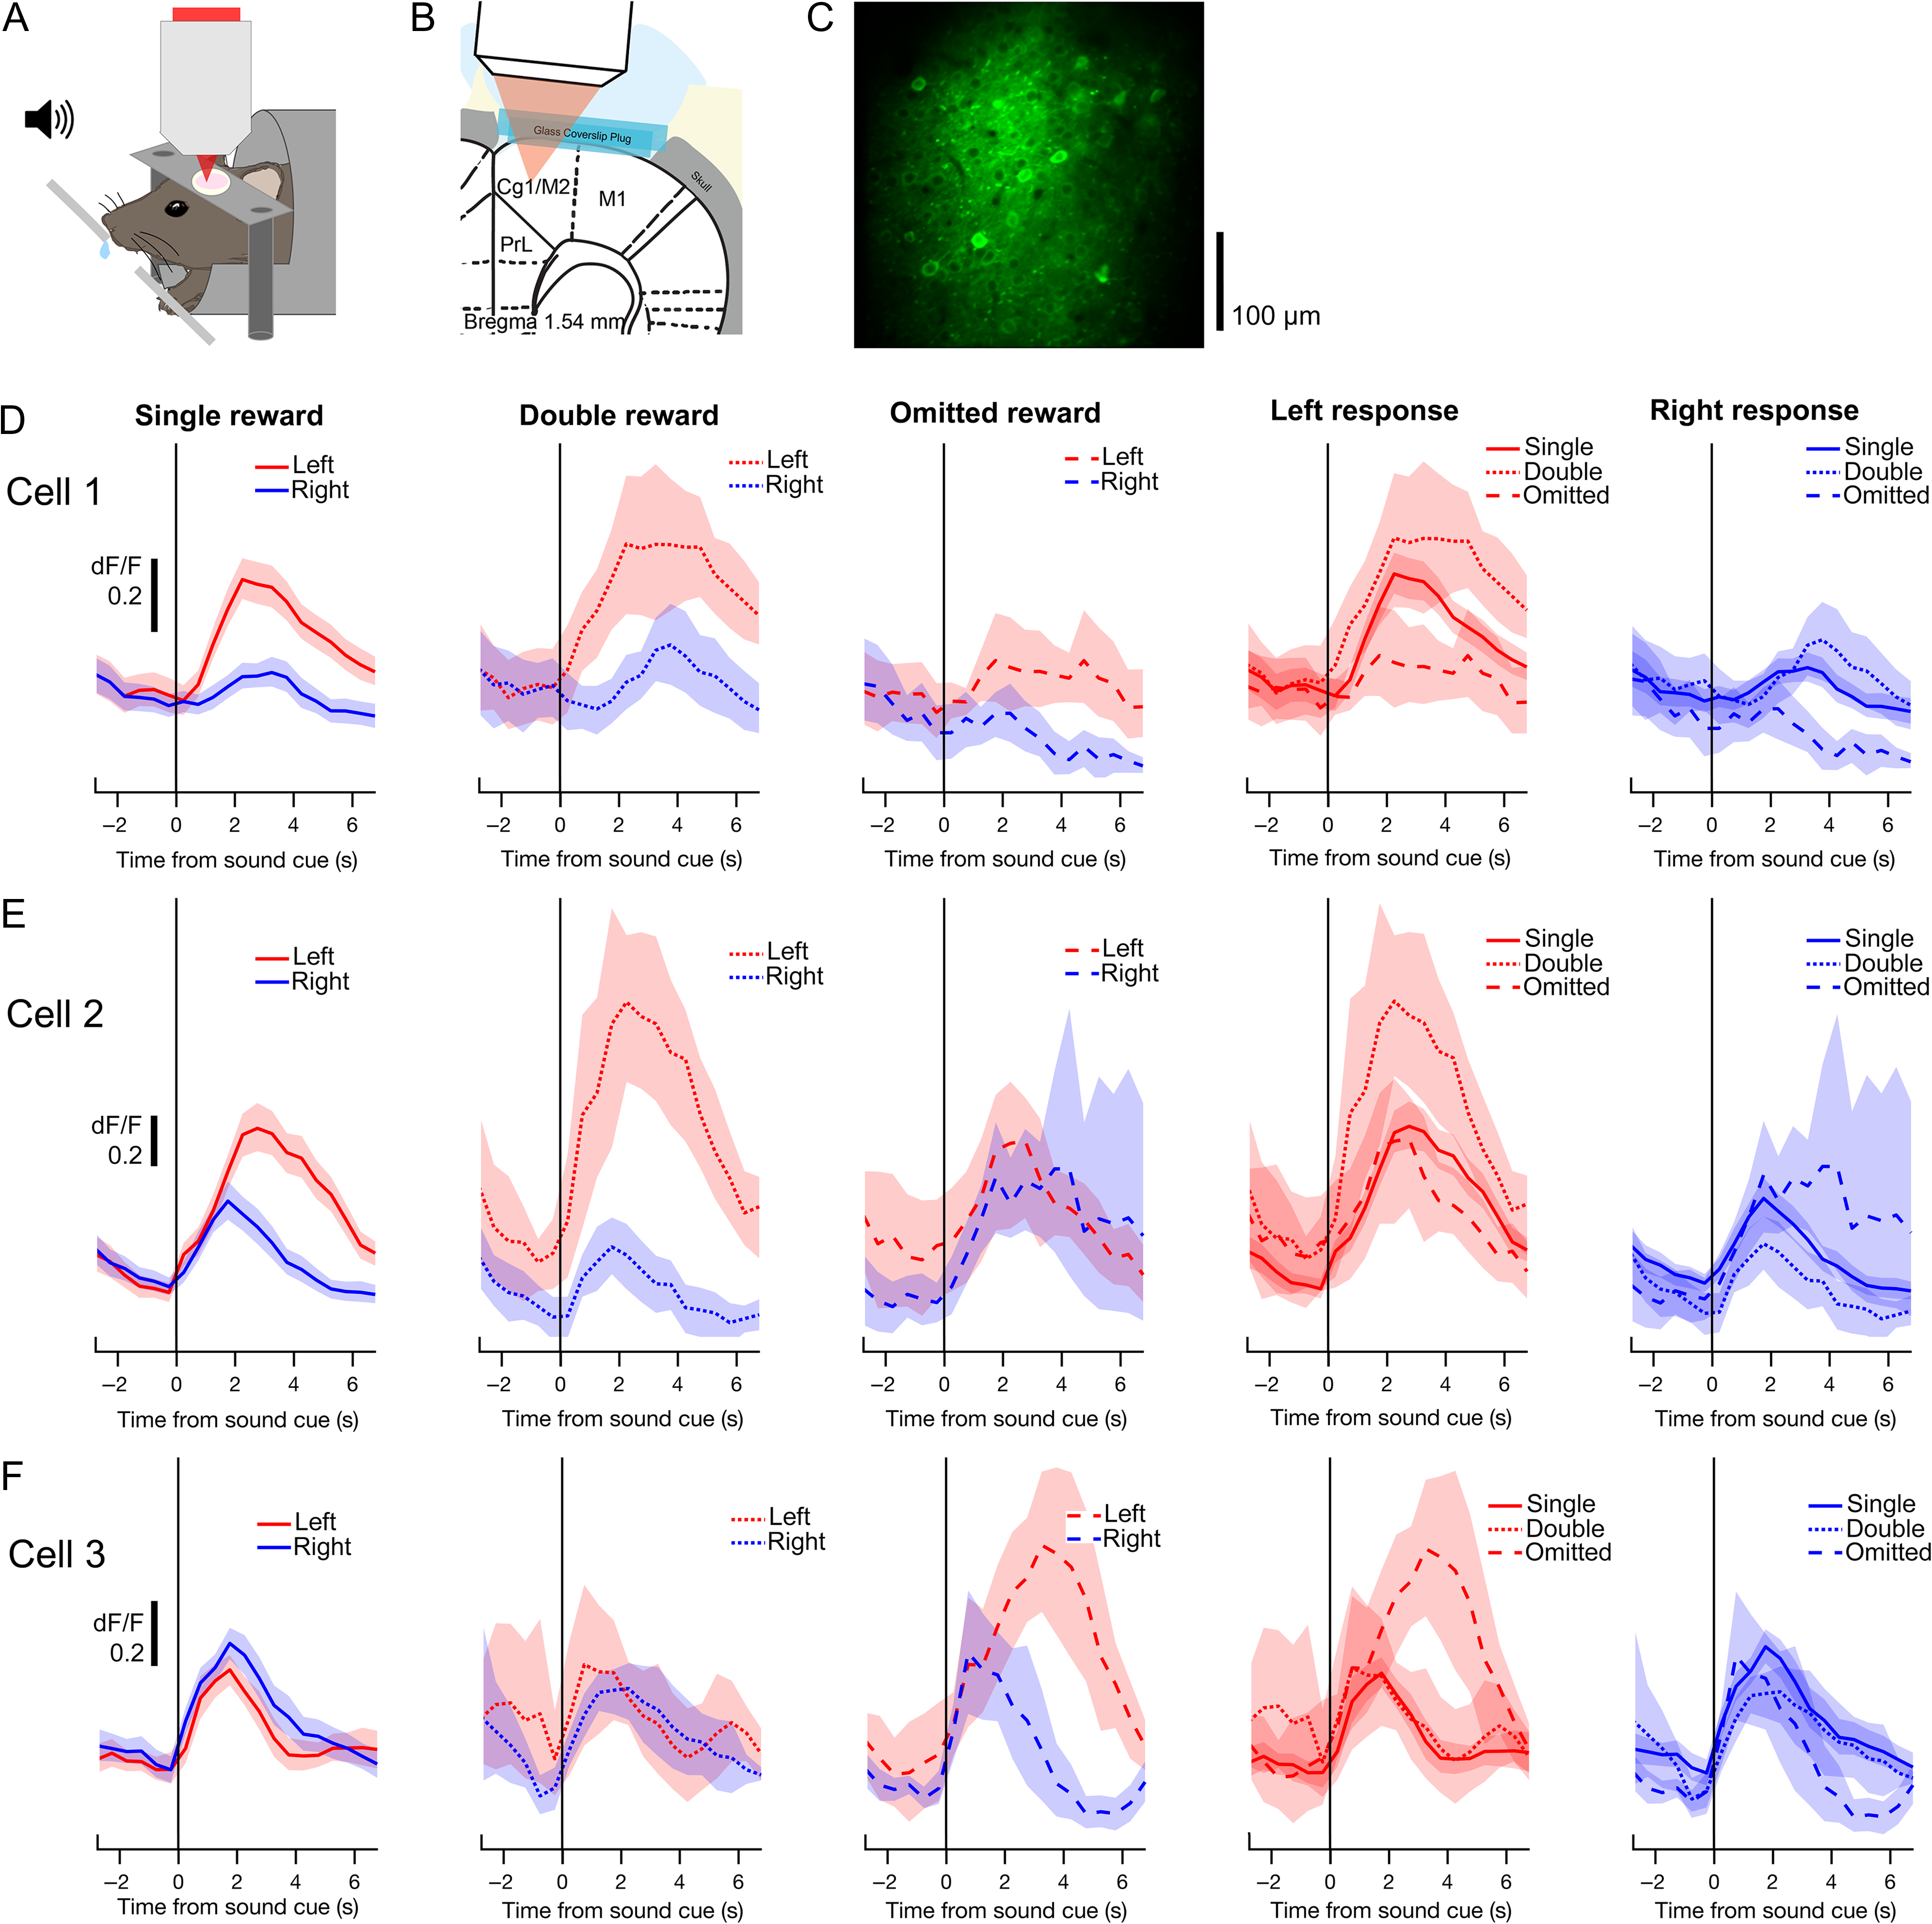
\includegraphics[width=\textwidth]{Figures/Chapter2/CC_fig3} 
\end{center}

\caption[Two-photon Ca\textsuperscript{2+} imaging of choice- and outcome-related signals]
{Two-photon calcium imaging of choice- and outcome-related signals in secondary motor cortex (M2). (A) Schematic representation of experimental setup for behavior with simultaneous two-photon imaging. (B) Schematic representation of preparation for in vivo two-photon imaging of M2. PrL, prelimbic cortex; Cg1, cingulate area 1; M1, primary motor cortex. (C) An example field-of-view in layer 2/3 of M2 containing GCaMP6s-expressing neurons. The image is a mean projection of the full time-lapse image stack from Experiment 13 in Table 1. (D) Mean fluorescence traces from an example cell, aligned to the sound cue and averaged across different subsets of trials. In the leftmost three panels, traces from left (red) and right (blue) trials are overlaid for each trial outcome. The rightmost two panels display the same data, with traces from single- (solid), double- (dotted) and omitted-reward trials (dashed) overlaid for each chosen action. Shading, 90\% confidence interval. (E–F) Same as D for two additional cells.}

\label{fig:CC_fig3}
\end{figure}